\documentclass[twoside,11pt]{article}
\usepackage{amsmath}
\usepackage{style}
\usepackage{booktabs}
\usepackage{longtable}
\usepackage{array}
\usepackage[table]{xcolor}
\usepackage{hyperref}
\usepackage{enumitem}
\usepackage{textcomp}
\usepackage{amsmath}
\usepackage{amssymb}

% Math notation shortcuts used throughout the manuscript
\newcommand{\ind}{\mathbb{I}}
\newcommand{\bx}{\mathbf{x}}

% Custom assumption environment
\newenvironment{assumption}[1][]{\vspace{0.5em}\noindent\textbf{Assumption#1:} \itshape}{\vspace{0.5em}}

% ── Table column types ────────────────────────────────────────────────────────
\newcolumntype{L}[1]{>{\raggedright\arraybackslash}p{#1}}
\newcolumntype{C}[1]{>{\centering\arraybackslash}p{#1}}

% ── Row shading color ─────────────────────────────────────────────────────────
\definecolor{rowgray}{gray}{0.93}

\ShortHeadings{
%% short title here
Bayesian Discrete-Time Modeling
}{
% last name
Kurth}
\firstpageno{1}

\begin{document}

\title{	Bayesian Discrete-Time Survival Modeling with Sensitivity Analysis for Informative Censoring: An Application to ICU Mortality\\
\vspace{.1in}
PHP2530
}


\author{ Adam M. Kurth}

\maketitle
\date{4 }


% =============================================================================
\section{Introduction} \label{sc:intro}
% =============================================================================


Accurate mortality risk profiling in the Intensive Care Unit (ICU) is essential for clinical decision-making, resource allocation, and the design of adaptive treatment strategies. Standard continuous-time approaches such as the Cox Proportional Hazards model remain dominant in biomedical survival analysis. However, when applied to large-scale electronic health records such as MIMIC-III \citep{PhysioNet-mimiciii-1.4}, handling of censoring is often treated as an unexamined formality. Cox and discrete-time models typically rely on the non-informative censoring assumption, meaning that the censoring mechanism (e.g., hospital discharge) carries no information about the underlying survival process beyond what is captured by observed covariates \citep{kalbfleisch2003statistical}.

In the ICU context, this assumption is immediately suspect. A patient that is ``censored'' is the result of a purposeful clinical decision. This clinically determined process is likely to be systematically related to the patient's underlying health status and mortality risk. Thus, this dependence between the censoring \(C_i\) and the unobserved failure process \(T_i\) violates the standard assumption and biases downstream inference of hazard estimates, coefficient effects, and predicted survival functions.

The consequences of informative censoring have been studied in the missing data literature. \citet{rubin1976} formalized the missingness taxonomy that maps directly to censoring. The main interest here is the consequences of violations to the Missing at Random (MAR) assumption, which corresponds to the non-informative censoring assumption. Further, \citet{tsiatis1975} shows a fundamental identifiability issue: from the observed data \((y_i, \delta_i)\) alone, the marginal distributions of \(T_i\) and \(C_i\) cannot be identified without structural assumptions on their joint distribution. This means that diagnostics based on the observed data alone cannot distinguish informative from non-informative censoring. Any assessment of the censoring mechanism must rely on untestable structural assumptions, thus motivating the need for sensitivity analyses.

The central question of this project is: \textit{under what conditions does the independent right-censoring assumption hold in ICU survival data, and what are the consequences for Bayesian posterior inference when it is violated?} We address this question through three methodological contributions, all developed within a discrete-time Bayesian framework using the person-period formulation of \citet{allison-discrete}.

First, we formalize the independent censoring assumption within the context of missing data, derive the standard discrete-time likelihood factorization, and characterize the consequences of violations to this assumption (Section~\ref{sc:naive-likelihood}). Second, we develop a \emph{sensitivity analysis} following the selection model approach of \citet{scharfstein1999}, which introduces a fixed sensitivity parameter \(\gamma\) that indexes the log-odds ratio of mortality between patients who are censored and those who remain under observation (Section~\ref{sc:sensitivity}). By finding the \emph{tipping point} \(\gamma^\ast\) at which critical clinical conclusions change, we provide a principled way to evaluate the robustness of our findings to departures from independent censoring. Third, we examine a \emph{shared frailty model} that introduces a patient-level random effect \(b_i\) to capture unobserved heterogeneity that may confound both the censoring decision and the mortality process (Section~\ref{sc:frailty}). Through a simulation study (Appendix~\ref{app:simulation}), we demonstrate that continuous patient-level frailty is weakly identified from sparse binary panel data with daily discretization, motivating the sensitivity analysis as the more principled approach.

The computational backbone uses Hamiltonian Monte Carlo (HMC) via Stan \citep{stan-software, hoffman-gelman-nuts} for the primary analysis, complemented by the P\'olya-Gamma data augmentation scheme \citep{polya-gamma} for conjugate Gibbs sampling of the logistic hazard model (Section~\ref{sc:computation}). A simulation study calibrating these methods against known data-generating processes is presented in Appendix~\ref{app:simulation}.


%=============================================================================
\section{Data Structure, Person-Period Format, \& Notation}\label{sc:notation}
% =============================================================================

% expand upon this for write-up
Let $i = 1, \dots, N$ index unique ICU admissions from MIMIC-III. We define:
\begin{itemize}[noitemsep]
  \item $T_i > 0$: the latent time to in-hospital death (continuous, in days).
  \item $C_i > 0$: the censoring time, defined as the time of hospital discharge if the patient does not die, i.e., the time at which the patient leaves the study for any reason, alive. In MIMIC-III, this is a clinically determined event, not an administrative one.
  \item $y_i = \min(T_i, C_i)$: the observed follow-up time (days).
  \item $\delta_i = \ind(T_i \le C_i)$: failure indicator.
  \item $\bx_i \in \mathbb{R}^P$: a vector of static baseline covariates (age, admission type, comorbidity scores, etc.), measured at time-zero (ICU admission).
\end{itemize}


\paragraph{Discretization.}
% PRIMARY ANALYSIS: 
%   - WEEK-LENGTH INTERVALS (\(\Delta = 7\) days, \(K \approx 4 - 5\) intervals for 70-day follow-up)
% SENSITIVITY ANALYSIS: 
% 1. BI-WEEKLY INTERVALS (\(\Delta = 14\) days, \(K=5\)) AND 
% 2. DAY-LENGTH INTERVALS (\(\Delta = 1\) day, \(K=70\))
We partition continuous time into discrete intervals of width \(\Delta\):  The intervals are, \([0,\Delta), [\Delta, 2\Delta), \dots, [(K-1)\Delta, K\Delta)\) with \(t = 1, \dots, K\) indexing those intervals. The discrete time failure time is \(T_i = \lceil T_i / \Delta \rceil\) and similarly the discrete censoring time is \(C_i = \lceil C_i / \Delta \rceil\). Our primary analysis will use week-length intervals (\(\Delta = 7\) days), yielding \(K \approx 4 - 5\) intervals. To assess sensitivity to this choice, we will also explore bi-weekly intervals (\(\Delta = 14\) days, \(K=5\)) and day-length intervals (\(\Delta = 1\) day, \(K=70\)) in Section~\ref{sc:sensitivity}. The finer the discretization, the better the approximation to the underlying continuous-time process, but the larger the dataset and more parameters to estimate.


\paragraph{Person-Period expansion.}
The data is restructured into a ``person-period" format \citep{allison-discrete}, so that patient \(i\) contributes one row per interval \(t=1,\dots, \tilde{y}_i\), yielding the binary outcome: 

\begin{equation}
    y_{i,t} = \ind\left( T_i \in [(t-1)\Delta, t\Delta), \delta_i = 1\right)  
        = \begin{cases}
            1 & \text{if patient $i$ dies in interval $t$} \\
            0 & \text{otherwise}
        \end{cases}
\end{equation}
Censored pateints contribute \(y_{i,t} = 0\) for \(t=1,\dots, \tilde{C}_i\) and are removed from the risk set thereafter. Patients who die contribute \(y_{i,t} = 1\) for \(t=1,\dots, \tilde{T}_i\) and exit. The total number of persion-period rows is \(\mathcal{R} = \sum_{i=1}^N \tilde{y}_i\).

% =============================================================================
\section{Standard Likelihood \& Censoring Assumption} \label{sc:naive-likelihood}
% =============================================================================
Here, I will introduce the standard likelihood and assess the direct impacts under violations of the independent censoring assumption. This will motivate the need for the frailty model and sensitivity analysis extensions in Sections~\ref{sc:frailty}--\ref{sc:sensitivity}. 

In \citep[Section 2.2]{kalbfleisch2003statistical}: the discrete-time Bernoulli likelihood for patient \(i\) is:
\begin{align} \label{eq:discrete-time-hazard}
    h_{i,t} 
    &= \Pr(Y_{i,t} = 1 \mid Y_{i,t-1} = 0, \bx_i)  = \Pr(T_i = t \mid T_i \ge t, \bx_i), \quad t = 1, \dots, K_i
\end{align}
for \(K_i\) being the last interval for which patient \(i\) is at risk (i.e., \(K_i = \tilde{y}_i\)). The corresponding survival function is: 
\begin{equation}
    S_i(t) = \Pr(T_i > t \mid \bx_i) = \prod_{s=1}^t (1 - h_{i,s})
\end{equation}


\subsection{Full Likelihood.}
Given right-censoring, the likelihood contribution for patient \(i\), involves the joint density of \((y_i, \delta_i)\) given \(\bx_i\), which in principle depends on the failure (parameters \(\boldsymbol{\theta}\)) and censoring processes (parameters \(\boldsymbol{\phi}\)). Let \(f_T, S_T,\) and \(f_C, S_C\) denote the densities and survival functions of \(T_i\) and \(C_i\). The full data likelihood is \citep[Section 3.2]{kalbfleisch2003statistical}:
\begin{equation}\label{eq:full-lik}
    \mathcal{L}_i^{\text{full}}(\boldsymbol{\theta}, \boldsymbol{\phi})
    = \bigl[f_T(y_i \mid \bx_i)\, S_C(y_i \mid \bx_i)\bigr]^{\delta_i}
      \bigl[S_T(y_i \mid \bx_i)\, f_C(y_i \mid \bx_i)\bigr]^{1 - \delta_i},
\end{equation}
This expression cannot be seperated into independent parts of \(\boldsymbol{\theta}\) and \(\boldsymbol{\phi}\) unless failure and censoring processes are conditionally idependent (i.e. \(T_i \perp C_i \mid \bx_i\)). This non-separability reflects the fundamental identifiability problem established by \citet{tsiatis1975}. He shows from infinitely many joint distributions of \((T_i, C_i)\) that are consistent with the observed data \((y_i, \delta_i)\). 


\subsection{Independent Censoring Assumption} \label{sc:indep-cens}
\begin{assumption}[][Independent Right-Censoring; K\&P Section~2.4]
  \label{assump:indep-cens}
  The censoring mechanism is \emph{non-informative} in the sense that:
  \begin{equation}
    T_i \perp C_i \;\mid\; \bx_i.
  \end{equation}
  Equivalently, at any time $t$ in which patient $i$ is under
  observation, knowing the exact censoring time $C_i$ provides no additional
  information about future survival beyond what $\bx_i$ already encodes.
\end{assumption}

\noindent
Under Assumption~\ref{assump:indep-cens}, the full likelihood \eqref{eq:full-lik} factors as: 
\begin{align}
    \mathcal{L}_i^{\text{full}} (\boldsymbol{\theta}, \boldsymbol{\phi}) 
    &= \underbrace{ \left[ f_{T}(y_i \mid \bx_i) \right]^{\delta_i} 
        \left[ S_T(y_i \mid \bx_i)\right]^{1-\delta_i} }_{\mathcal{L}_i(\boldsymbol{\theta}) }
        \underbrace{ 
            \left[ S_{C}(y_i \mid \bx_i) \right]^{\delta_i} 
            \left[ f_{C}(y_i \mid \bx_i) \right]^{1 - \delta_i} 
            }_{\substack{\text{depends only on } \boldsymbol{\phi} \text{ (under Assumption~\ref{assump:indep-cens}) }}}
\end{align} 
so that inference about \(\boldsymbol{\theta}\) can be processed using the observed-data likelihood \(\mathcal{L}_i(\boldsymbol{\theta})\) without any reference to the censoring mechanism (K\&P, Equation 3.1). In discrete-time person-period form:
\[
    \mathcal{L}(\boldsymbol{\theta}) 
    = \prod_{i=1}^N \prod_{t=1}^{K_i} h_{i,t}^{y_{i,t}} (1 - h_{i,t})^{1 - y_{i,t}}
\]
where each \((i,t)\) term is treated as an independent Bernoulli trial.

\subsection{Censoring Condition \& Operative Assumption} \label{sc:censoring-conditions}

Independent censoring (Assumption~\ref{assump:indep-cens}) corresponds to Missing at Random (MAR) in \citet{rubin1976}'s taxonomy of missing data. This means that conditional on \(\bx_i\), the censoring mechanism carries no information about \(T_i\). Since \(\bx_i\) contains only baseline measurements and MIMIC-III discharge decisions, are likely more reprepresentative using time-varying covarites, the MAR assumption is likely violated in the ICU context, and thus the censoring mechanism is likely informative to some degree. This motivates the operative censoring condition (Assumption~\ref{assump:operative-cens}), which is the working assumption that the MAR assumption is violated, and thus we will proceed with methods that account for the degree of informative censoring, such as the frailty model (Section~\ref{sc:frailty}) and the sensitivity analysis (Section~\ref{sc:sensitivity}).

\begin{assumption}[][Operative Censoring Condition] \label{assump:operative-cens}
    In our static covariate setting, MAR given only \(\bx_i\) is the operative censoring requirement. Because time-varying information is likely critical to drive discharge decisions, the censoring mechanism is likely informative (i.e., \(T_i \not\perp C_i \mid \bx_i\)). Thus, we will proceed under the assumption that the MAR assumption is violated, and work towards developing methods to account for this.
\end{assumption}

\subsection{Consequences of Informative Censoring}
When the independent censoring assumption fails, three consequences follow.


\paragraph{Biased Hazard Estimation.}
First, if the healthier patients are systematically discharged before sicker ones, the risk set at time \(t\) is biased towards sicker patients, inflating the observed hazard \(\hat{h}_t\) relative to the true marginal hazard \(h_t^\ast\). The risk set at time \(t\) is \(\mathcal{R}_t = \{i: y_i \geq t\} = \{i: T_i \geq t, C_i \geq t\}\) and \(\mathcal{C}_t = \{i: C_i < t\}\). The bias is (Appendix~\ref{app:biased-hazard}):
\begin{equation} \label{eq:bias-approx}
    \hat{h}_t \approx h_t^\ast + \frac{\lambda_t \Delta_t }{1-\lambda_t} \quad \text{where} \quad
    \hat{h}_t = \frac{ \sum_{i \in \mathcal{R}_t} \ind(T_i = t) }{ |\mathcal{R}_t| }
\end{equation}
where \(\lambda_t = |\mathcal{C}_t|/|\mathcal{R}_t|\) is the proportion of surviving patients censored by time \(t\), and \(\Delta_t > 0\) is the hazard difference between the full survivor population and the censored subgroup. The bias is positive for all \(\lambda_t, \Delta_t > 0\) and increases as \(\lambda_t \to 1\) (i.e. more patients are discharged over time, shrinking the risk set), and is the discrete-time analogue of the frailty-induced selection bias in the continuous-time setting \citep{vaupel1979,lancaster1979}. See Appendix~\ref{app:biased-hazard} for a full derivation of the bias in the observed hazard under informative censoring.

Since the observed hazard being positively biased in each interval, this implies that the estimated survival function \(\hat{S}(t) = \prod_{s=1}^t (1 - \hat{h}_s)\) will compound this bias and be systematically lower than the true marginal survival \(S^\ast(t)\). This means that patients with long ICU stays (e.g., 10+ days) will have their survival estimates show a large discrepancy from the true marginal survival. This leads to a pessimistic empirical estimate of survival.


\paragraph{Confounding Bias in Covariate Effects.}
Covariate information that might predict early discharge and lower mortality risk (e.g., elective admission, lower comorbidity scores) will have their effects \(\boldsymbol{\beta}\) confounded by the informative censoring process. Thus, estimand derived in the standard likelihood will no longer represent the pure effect of \(\bx_i\) on mortality risk, but rather both the effect of \(\bx_i\) on the failure and censoring processes. \citet{scharfstein1999} formalizes this as a failure of the semiparametric estimation equations when MAR is violated, where the score function for \(\boldsymbol{\beta}\) is biased proportional to the dependence between \(T_i\) and \(C_i\) given \(\bx_i\). This is formalized in Appendix~\ref{app:scharfstein1999}, where the bias in the score function for \(\boldsymbol{\beta}\) under informative censoring can be expressed as:
\begin{equation}  \label{eq:confounding-bias}
    \text{Bias}(\alpha) \approx -\alpha \, \mathbb{E} \Big[ \Lambda_0(C_i \mid \bx_i) \, T_i \, S_\text{full}(\boldsymbol{\beta}) \Big]
\end{equation}
In the context of this project, the full-data score (\(S_\text{full}(\boldsymbol{\beta})\)) is Equation~\ref{eq:full-lik}. This bias is driven by \(\alpha\) (the severity of the MAR violation/selection) and the covariance (cumulative hazard) between the failure time \(T_i\) and the censoring \(\Lambda_0(C_i \mid \bx_i)\). Because \(\alpha\) cannot be identified from the observed data alone, standard estimation fails.


\paragraph{Corrections.}
The consequences yield a upward systematic bias in observed hazards and a multiplicative bias in the score function for \(\boldsymbol{\beta}\). We address this through two complementary strategies. First, the sensitivity analysis in Section~\ref{sc:sensitivity} directly parameterizes the residual bias through \(\gamma\), allowing us to assess how large the MAR violation would need to be before changing clinical conclusions. Second, the shared frailty model (Section~\ref{sc:frailty}) partially restores the risk-set representativeness by conditioning on the unobserved heterogeneity \(b_i\), though our simulation study demonstrates that this approach faces identifiability challenges with sparse binary data. Thus, the sensitivity analysis is the more principled approach to account for informative censoring in this context, while the frailty model serves as a useful diagnostic and partial correction.



\section{Logistic Hazard Model} \label{sc:frailty}

The persion-period formulation in Section~\ref{sc:notation} recasts the discrete-time survival hazard as a first-order Markov chain on the state space \(\{1,0\}\) where \(0\) denotes ``alive'' and \(1\) denotes ``dead'' (an absorbing state). At each interval \(t\), a patient who survives to that point (\(Y_{i,t-1} = 0\)) either transitons to death (\(Y_{i,t} = 1\)) or remains alive (\(Y_{i,t} = 0\)). Note that conditioning on \(Y_{i,t-1} = 0\), also conditions on all previous time intervals while also satisfying the Markov property. The discrete-time hazard \eqref{eq:discrete-time-hazard} is precisely the one-step transition probability, which can be modeled as a Bernoulli GLMM with a logistic link. 

\subsection{Standard Model (Model A)}  \label{sc:standard-model} 
The primary analysis model specifies the hazard via a logistic link within interval-specific intercepts and shared covariate effects:
\begin{align}
    Y_{i,t} \mid h_{i,t} &\sim \text{Bernoulli}(h_{i,t}), \quad t = 1, \dots, K_i,\; i = 1, \dots, N, \label{eq:obs-model} \\
    \text{logit}(h_{i,t}) &= \alpha_t + \bx_i^\top \boldsymbol{\beta} 
    % = \mathbf{X}^\ast \boldsymbol{\theta}, \qquad \text{where } \mathbf{X}^\ast = \begin{bmatrix}\mathbf{I}_K & \mathbf{X}\end{bmatrix} \text{ and } \boldsymbol{\theta} = \begin{bmatrix}\boldsymbol{\alpha} \\ \boldsymbol{\beta}\end{bmatrix},
    \label{eq:link-standard}
\end{align}
with priors:
\begin{alignat}{2}
    \alpha_1 &\sim \mathcal{N}(0, \sigma_0^2), &\qquad&\text{(anchor)} \label{eq:alpha1-prior} \\
    \alpha_t \mid \alpha_{t-1} &\sim \mathcal{N}(\alpha_{t-1}, \sigma_\alpha^2), &\qquad& t = 2, \dots, K, \label{eq:rw-prior} \\
    \sigma_\alpha &\sim \text{Student-}t^+(3, 0, 1), \label{eq:sigma-alpha-prior} \\
    \boldsymbol{\beta} &\sim \mathcal{N}(\mathbf{0}, \tau^2 \mathbf{I}_P). \label{eq:beta-prior}
\end{alignat}

The first-order random walk prior on \(\boldsymbol{\alpha} = (\alpha_1, \dots, \alpha_K)^\top\) endosed the belief that neighboring intervals have similar baseline log-odds of death. As the risk set shrinks at later intervals, this prior borrows strength from adjacent time points, regularizing \(\alpha_t\) where data is sparse. The half Student-t prior on \(\sigma_\alpha\) is weakly infrmative, allowing for a wide range of temporal variability while still favoring smoother trajectories, and avoids boundary issues of the conjugate Inverse-Gamma prior with small shape parameters \citep{gelman-prior-2006}.  We set \(\sigma_0^2 = \tau^2 = 10\) as weakly informative defaults. 

Let \(\boldsymbol{\theta} = (\boldsymbol{\alpha}^\top, \boldsymbol{\beta}^\top)^\top \in \mathbb{R}^{K + P}\) denote the combined fixed-effect vector. This model is well identified and converges reliably under HMC. Appendix~\ref{app:simulation} demonstrates ESS in the thousandds for all \(\beta_j\) and zero-divergences across all configurations. Under the independent censoring assumption, Model A provides the best posterior inference for the marginal hazard and covariate effects.


% STOPPED HERE

\subsection{Frailty Extension (Model B)} \label{sc:frailty}
To capture unobserved patient-level heterogeneity, we extend Model A with a Gaussain random effect \(b_i\) (frailty) for each patient \(i\):
\begin{align}
    \text{logit}(h_{i,t}) &= \alpha_t + \bx_i^\top \boldsymbol{\beta} + b_i 
    \label{eq:link-frailty}
\end{align}
with additional priors:
\begin{alignat}{2}
    b_i &\sim \mathcal{N}(0, \sigma_b^2), &\qquad& i = 1, \dots, N,\label{eq:frailty-prior} \\
    \sigma_b &\sim \text{Exponential}(1). \label{eq:sigma-b-prior}
\end{alignat}

the penalized complexity (PC) prior as a standard exponential, favors smaller \(\sigma_b^2\) \citep{simpson-pc-priors} which shrinks towards no heterogeneity \(b_i = 0\) which is the base model (Model~A). This is more principled than the Inverse-Gamma hyperprior for this setting, as it avoids both the small shape parameter placing excessive mass near zero and having heavy right tails. 


\paragraph{Why Frailty Addresses Informative Censoring.}
The frailty term \(b_i\) captures heterogeneity that may drive both discharge decisions and mortality risk. By conditioning on the random effect, the model weakens the censoring requirement to:
\begin{equation} \label{eq:frailty-indep-cens}
    T_i \perp C_i \;\mid\; \bx_i, b_i
\end{equation}
This is a strictly weaker condition than Assumption~\ref{assump:indep-cens}, requiring only that the augmented covariate set \((\bx_i, b_i)\) renders censoring non-informative \citep[Chapter~7]{daniels2008}. Under \eqref{eq:frailty-indep-cens}, the conditional analogue of the bias term in \eqref{eq:bias-approx} vanishes.



An important caveat is that the bias formula in \eqref{eq:bias-approx} assumes \(\Delta_t > 0\), meaning censored patients are healthier. In the ICU context, this is likely an oversimplification. While the majority of patients are likely to improve \(b_i < 0\), those who are discharged to hospice for example, might have a worse prognosis \(b_i > 0\). For these patients, \(h_t^c > h_t^\ast\) locally, attenuating or even reversing the bias. The frailty model handles this naturally by estimating \(b_i\) individually. But whether \eqref{eq:frailty-indep-cens} holds is ultimately untestable, which is why the sensitivity analysis in Section~\ref{sc:sensitivity} remains essential.


\paragraph{Identifiability Limitations.}
The baseline hazard \(\alpha_t\) and frailties \(b_i\) are seperately identified by the temporal structure of the data. The random walk \(\alpha_t\) varies across intervals and \(b_i\) by correlation across intervals \emph{within} patient \(i\). However, patients observed for few intervals (or no intervals) contribute little within-patient information, and their \(b_i\) posteriors are dominated by the prior, shrinking toward zero.


Our simulation study in Appendix~\ref{app:simulation} reveals a fatal weakness: within \(N\) patients contributing on average \(\bar{K}\) person-period rows each, the \(N\) random effects are weakly identified from the sparse binary data. The frailty variance \(\sigma_b^2\) consistently exhibits low effective sample sizes (ESS \(\approx 80--150\) from 10,000 posterior draws), \(\hat{R} > 1.01\), and instability across discretization grids. Model B never improves upon Model A in leave-one-out cross-validation (LOO-CV), confirming that the data does not support these extra parameters. 

%=============================================================================
\subsection{Sensitivity Analysis for Informative Censoring} \label{sc:sensitivity}
%==============================================================================
The sensitivity analysis on Model A and frailty model address complementatry aspects of informative censoring. Frailty \(b_i\) models heterogenity \emph{parametrically}, assuming the Gaussian prior \eqref{eq:frailty-prior} and condition \eqref{eq:frailty-indep-cens}. The sensitivity analysis, by contrast,  \emph{nonparametrically} probes the robustness of conclusions by indexing departures from independent censoring without specifying a particular dependency structure. Our simulation (Appendix~\ref{app:simulation}) demonstrates that the sensitivity analysis is well-identified and converges cleanly at all values of \(\gamma\), whereas the frailty model suffers from weak identifiability. For this reason, the sensitivity analysis serves as the primary tool for assessing informative censoring in the MIMIC-III analysis.
 
\subsection{The Selection Model} \label{sc:selection-model}
Following \citet{scharfstein1999} and the Bayesian treatment of \citet{daniels2008}, define \(\gamma\) as the log-odds ratio of death at time \(T_i = t\) between patients censored at \(t\) and those remaining under observation at \(t\):
\begin{equation}
    \gamma = \log\left( \frac{\Pr( T_i = t \mid T_i \geq t, C_i = t, \bx_i)}{\Pr( T_i = t \mid T_i \geq t, C_i > t, \bx_i)} \right)
\end{equation}
\(\gamma = 0\) corresponds to non-informative censoring (MAR), \(\gamma < 0\) means censored patients have lower mortality risk (discharge reflects improvement), and \(\gamma > 0\) means censored patients have higher mortality risk (discharge reflects deterioration or transfer to hospice). Here, \(\gamma\) plays the role of the selection parameter ``\(\alpha\)'' in \eqref{eq:confounding-bias}, indexing the residual selection bias that cannot be captured by the observed covariates \(\bx_i\) alone. Unlike the frailty variance \(\sigma_b^2\), \(\gamma\) is not estimated from the data but rather swept over a grid, making the analysis immune to identifiability problems.

Note that we conduct the sensitivity analysis on Model A and therefore do not condition on \(b_i\). When \(b_i\) is included, the sensitivity parameter would index the \emph{residual} selection bias beyond what the frailty captures; with Model~A, it indexes the \emph{total} departure from MAR.



\subsection{Tilted Likelihood}
Under the selection model, the hazard for censored observations at the terminal interval is adjusted by an exponential tilting factor:
\begin{equation}\label{eq:tilted-hazard}
    \mathrm{logit}(\tilde{h}_{i,t}) = \mathrm{logit}(h_{i,t}) + \gamma \ind(C_i = t, \delta_i = 0), \qquad \text{ where } \delta_i = \ind(T_i \le C_i)
\end{equation}
Equivalently, the mortality odds are multiplied by \(\exp(\gamma)\) at the censoring interval. For uncensored observations and non-terminal intervals, \(\tilde{h}_{i,t} = h_{i,t}\). The tilted likelihood is:
\begin{equation} \label{eq:tilted-lik}
    \tilde{\mathcal{L}}(\boldsymbol{\theta}; \gamma) = \prod_{i=1}^N \prod_{t=1}^{K_i} \tilde{h}_{i,t}^{y_{i,t}} (1 - \tilde{h}_{i,t})^{1 - y_{i,t}}
\end{equation}

The tilted likelihood is a reweighting of the original likelihood, where the contribution of censored observations at their terminal interval is adjusted by \(\gamma\). This allows us to assess how sensitive our inferences are to departures from the MAR assumption by varying \(\gamma\) and observing how the posterior distributions of parameters and survival curves change.
The mortality odds are:
\begin{equation}\label{eq:odds-tilt}
    \frac{ \tilde{h}_t }{ 1 - \tilde{h}_t } = \frac{ h_t }{ 1 - h_t } \cdot \exp(\gamma) \quad \text{if } C_i = t, \delta_i = 0
\end{equation} 

Since \(\gamma\) is fixed for each sweep and the censoring indicator \(\ind(C_i = t, \delta_i = 0)\) is observed, the tilt term \(o_{i,t} = \gamma \ind(C_i = t, \delta_i = 0)\) is a known offset for each person-period row. The tilted linear predictor is:
\begin{equation}
    \tilde{\eta}_{i,t} = \alpha_t + \bx_i^\top \boldsymbol{\beta} + o_{i,t}
\end{equation}
This is simply Model~A with a known offset added at censoring times. The offset does not introduce any new parameters to estimate, so the tilted model inherits the excellent convergence properties of the standard model. 

\subsection{Protocol.}


Following \citet{daniels2008}:
\begin{enumerate}[noitemsep, topsep=0pt]
    \item Fit the standard model (Model~A) with $\gamma = 0$ and record posterior
      summaries of $\boldsymbol{\beta}$, $\sigma_\alpha$, and $\hat{S}(t \mid \bx)$.
    \item Select a grid
      $\gamma \in \{-2.0, -1.5, -1.0, -0.5, -0.25, 0, 0.25, 0.5, 1.0, 1.5, 2.0\}$, where
      negative values correspond to the clinically plausible
      direction (healthier patients discharged earlier).
    \item For each $\gamma$, refit Model~A with the tilted likelihood~\eqref{eq:tilted-lik}.
    \item Report posterior means and 95\% credible intervals for each $\beta_j$
      as a function of $\gamma$ (sensitivity plot).
    \item Identify the tipping point $\gamma^\ast_j$ for each covariate: the value at which the
      95\% credible interval for $\beta_j$ first includes zero.
\end{enumerate}


If conclusions are robust across the grid of \(\gamma\), the standard analysis assuming MAR is sufficient, despite the potential for informative censoring. If conclusions change at modest values of \(|\gamma|\), this quantifies the fragility of the findings. 


% =============================================================================
\section{Computation} \label{sc:computation}
% =============================================================================


The initial motivation for the project was to build the frailty model under the Polya-Gamma (PG) data augmentation scheme of \citet{polya-gamma} to leverage conjugacy for efficient Gibbs sampling in large datasets. However, this approach necessitates an exact likelihood specification and under informative censoring, the likelihood we assumed is not entirely correct. In running the initial analyses on MIMIC-III, the frailty PG sampler (in its centered parameterization) \((b_i, \sigma_b^2)\) exhibited Neal's funnel geometry \citep{neal-funnel}— meaning that for small \(\sigma_b^2\), \(b_i\) was tightly concentrated about zero and mixed well, but for large \(\sigma_b^2\), \(b_i\) had was diffuse and the sampler struggled to explore the posterior, manifesting in very low ESS. 

\subsection{Hamiltonian Monte Carlo via Stan}\label{sc:stan}

To address the funnel geometry, we implement the frailty model in Stan \citep{stan-software} using the No-U-Turn Sampler (NUTS; \citealp{hoffman-gelman-nuts}), a self-tuning variant of Hamiltonian Monte Carlo (HMC). The key improvement is a \emph{non-centered} reparameterization:
\begin{equation}\label{eq:non-centered}
    b_i^{\text{raw}} \sim \mathcal{N}(0, 1), \qquad b_i = \sigma_b \cdot b_i^{\text{raw}},
\end{equation}
which decouples the sampling of \(b_i\) and \(\sigma_b\). Combined with PC prior \eqref{eq:sigma-b-prior} this yields substantially better mixing. 



\subsection{Computational Comparison}
SECTION SHOULD DISCUSS REAL RESULTS INSTEAD OF SIMULATION STUDY.


The simulation study in Appendix~\ref{app:simulation} provides a head-to-head comparison:
\begin{itemize}[noitemsep]
    \item \textbf{PG Gibbs (centered)}: Efficient for the standard model, but ESS(\(\sigma_b^2\)) \(\approx 14\) for the frailty model due to Neal's funnel. Useful as a pedagogical baseline.
    \item \textbf{Stan NUTS (non-centered)}: ESS(\(\sigma_b\)) \(\approx 140\), \(\hat{R} \approx 1.04\). Substantially better but still marginal for the frailty variance, reflecting weak identifiability rather than sampler inadequacy.
    \item \textbf{Model~A (standard) in Stan}: ESS \(> 5{,}000\) for all \(\beta_j\), \(\hat{R} \approx 1.00\), zero divergences. This is the recommended configuration for the MIMIC-III analysis.
\end{itemize}

The practical recommendation is to use Stan with Model~A for the primary analysis and the sensitivity sweep, and to present the frailty model (Model~B) as supporting evidence for the presence of unobserved heterogeneity. The PG Gibbs sampler serves as a methodological comparison demonstrating the computational consequences of centered vs.\ non-centered parameterizations.



% =============================================================================
\section{Application to MIMIC-III} \label{sc:application}
% =============================================================================





\newpage







% =============================================================================
\section{Discussion} \label{sc:discussion}
% =============================================================================

[To be completed. Key points to address:]

\paragraph{Summary of Contributions.}
This work makes three contributions to the analysis of ICU survival data under potentially informative censoring. First, we formalize the connection between the independent censoring assumption and the MAR framework, deriving explicit bias formulas for both hazard estimation and covariate effects. Second, we develop and validate a sensitivity analysis protocol based on exponential tilting that provides clinically interpretable tipping points for each covariate. Third, through a comprehensive simulation study, we demonstrate that continuous patient-level frailty is weakly identified from discrete-time survival data, providing principled justification for the sensitivity analysis approach over direct frailty estimation.

\paragraph{Limitations.}
The standard model uses only static baseline covariates. Time-varying covariates (e.g., daily lab values, vasopressor dosing) are likely informative for both mortality and discharge decisions, and their inclusion could reduce the degree of informative censoring. The sensitivity analysis assumes a constant \(\gamma\) across all censoring times and patient profiles; in practice, the selection mechanism may vary by time and patient characteristics. Extensions to covariate-dependent \(\gamma(\bx_i)\) are possible within this framework but increase the dimensionality of the sensitivity grid.

\paragraph{Future Work.}
Competing risks (e.g., death vs.\ discharge to home vs.\ transfer to another facility) represent a natural extension. In the discrete-time framework, this corresponds to a multinomial rather than Bernoulli observation model at each interval, with separate hazards for each competing event. The exponential tilting framework can be extended to this setting by introducing event-specific sensitivity parameters.





\appendix



\newpage
\section{Semiparametric Estimation Equations under Informative Censoring} \label{app:scharfstein1999}

Reiterating a key result from \citet{scharfstein1999} that pertains to this project, censoring induced confounding bias is a failure of the semiparametric estimation equations (score) for \(\boldsymbol{\beta}\) when the MAR assumption is violated. When the probability of censoring depends on the unobserved outcome (the failure time \(T_i\)), this constitutes a Missing Not at Random (MNAR) or nonignorable censoring mechanism. In this case, the standard score functions used to estimate \(\boldsymbol{\beta}\) are biased proportional to the dependence between \(T_i\) and \(C_i\) given \(\bx_i\).

Let \(\Delta_i = \ind(T_i \le C_i)\) be the observation indicator (0 if censored, 1 if observed). A standard solution under MAR to account for missing data is to use an Inverse Probability Weighting (IPW). If MAR holds, the probability of being observed depends only on \(\bx_i\), denoted \(\pi(\bx_i; \alpha = 0) = \Pr(\Delta_i = 1 \mid \bx_i)\). When MAR is violated, the true probability of being observed depends on both \(T_i\) and \(\bx_i\), denoted \(\pi(T_i, \bx_i; \alpha) = \Pr(\Delta_i = 1 \mid T_i, \bx_i)\). Again, \(\alpha\) is a non-identifiable selection parameter that indexes the severity of the MAR violation.

In standard parametric estimation, the expectation of the score at the true parameter value \(\boldsymbol{\beta}_0\) always equals zero. Under informative censoring, however, this is no longer the case. To find the bias, we take the expectation under the MNAR distribution:

\begin{align*}
    \mathrm{Bias}(\alpha)
    &= \mathbb{E} \left[ \frac{ \Delta_i }{\pi(\bx_i; 0)} S_\text{full}(\boldsymbol{\beta}_0) \right] 
    = \mathbb{E} \left[ \mathbb{E} \left[ \frac{ \Delta_i  }{\pi(\bx_i; 0)} S_\text{full} (\boldsymbol{\beta}_0) \bigg| T_i, \bx_i \right] \right]
    = \mathbb{E} \left[ \frac{\pi(T_i, \bx_i; \alpha)}{\pi(\bx_i; 0)} S_\text{full}(\boldsymbol{\beta}_0) \right]
\end{align*}
where \(S_\text{full}(\boldsymbol{\beta})\) is the full-data score function (i.e., the score function we would have if we observed \(T_i\) for all patients). Following \citet{scharfstein1999}, if we specify the conditional hazard of censoring as \(\lambda_C(t \mid \bx_i, T_i) = \lambda_0(t \mid \bx_i)\exp(\alpha T_i)\), where \(\lambda_0\) is the baseline hazard of censoring, and \(\exp(\alpha T_i)\) is the ``tilt'' caused by unobserved dependence between \(T_i\) and \(C_i\). The survival function of censoring at \(T_i\): \(\pi(T_i, \bx_i; \alpha) = \exp\{ - \int_0^{T_i} \lambda_C(u \mid \bx_i, T_i) du \}  = \exp\{ - \int_0^{T_i} \lambda_0(u \mid \bx_i) \exp(\alpha T_i) du \} = \exp\{ - \exp(\alpha T_i) \Lambda_0(T_i \mid \bx_i) \}\), where \(\Lambda_0\) is the cumulative baseline hazard of censoring. While under MAR, \(\pi(\bx_i; 0) = \exp\{ - \Lambda_0(T_i \mid \bx_i) \}\). Thus, the ratio of the true to assumed selection probabilities is:
\begin{align*}
    \frac{\pi(T_i, \bx_i; \alpha)}{\pi(\bx_i; 0)} 
    &= \frac{\exp\{ - \exp(\alpha T_i) \Lambda_0(T_i \mid \bx_i) \}}{\exp\{ - \Lambda_0(T_i \mid \bx_i) \}} \\
    &\approx \frac{\exp\{ - (1 + \alpha T_i) \Lambda_0(T_i \mid \bx_i) \}}{\exp\{ - \Lambda_0(T_i \mid \bx_i) \}}\\
     &= \exp\{ - \alpha T_i \Lambda_0(T_i \mid \bx_i) \}
\end{align*}
where \(e^{\alpha T_i} \approx 1 + \alpha T_i\) in the tilt term on the numerator. Applying a first-order Taylor expansion for small \(\alpha\) yields:
\begin{equation}
    \frac{\pi(T_i, \bx_i; \alpha)}{\pi(\bx_i; 0)} \approx 1 - \alpha T_i \Lambda_0(T_i \mid \bx_i)
\end{equation}
Substituting this back into the expectation yields the explicit bias approximation:
\begin{equation}
    \text{Bias}(\alpha) \approx -\alpha \, \mathbb{E} \Big[ \Lambda_0(T_i \mid \bx_i) \, T_i \, S_\text{full}(\boldsymbol{\beta}) \Big]
\end{equation}

This result explicitly demonstrates the main theoretical consequence of informative censoring: the bias in estimating \(\boldsymbol{\beta}\) is strictly driven by \(\alpha\) (the severity of the MAR violation/selection) and the covariance (cumulative hazard) between the failure time \(T_i\) and the censoring \(\Lambda_0(T_i \mid \bx_i)\). Because \(\alpha\) cannot be identified from the observed data alone, standard estimation fails, motivating the need for alternative approaches such as sensitivity analyses or frailty models (as discussed in Section \ref{sc:frailty}) to absorb this unobserved dependence. HOW TO CONNECT THIS TO THE FRAILTY MODEL/GLMM?





\section{Derivation of Biased Hazard under Informative Censoring} \label{app:biased-hazard}

At time \(t\), the full population of survivors decomposes into those in the risk set \(\mathcal{R}_t = \{i : T_i \geq t, C_i \geq t\}\) and those in \(\mathcal{C}_t = \{i : T_i \geq t, C_i < t\}\) who have been censored by \(t\), i.e. \(\mathcal{S}_t = \mathcal{R}_t \cup \mathcal{C}_t\). 

The true marginal hazard (\(h^\ast_t\)) and observed hazard (\(\hat{h}_t\)) are then:
\begin{align*}
    h^\ast_t &= \Pr(T_i = t \mid T_i \geq t)  
            = \mathbb{E}(h_{i,t} \mid T_i \geq t)\\
    \hat{h}_t &= \Pr(T_i = t \mid T_i \geq t, C_i \geq t)  
            = \mathbb{E}(h_{i,t} \mid T_i \geq t, C_i \geq t) 
            = \mathbb{E}(h_{i,t} \mid i \in \mathcal{R}_t)
\end{align*} 
\noindent
Introduce \(\lambda_t = \Pr(C_i < T_i \mid T_i \geq t) = |\mathcal{C}_t|/|\mathcal{R}_t|\) as the proportion of survivors (censored at \(t\)) relative to the risk set. Then, \(\hat{h}_t\) can be expressed as a mixture of the hazards in \(\mathcal{R}_t\) and \(\mathcal{C}_t\). Let \(h^c_t = \mathbb{E}(h_{i,t} \mid i \in \mathcal{C}_t)\) be the mean hazard among those censored by \(t\). Then:
\begin{align*}
    h^\ast_t &= (1-\lambda_t) \underbrace{ 
            \mathbb{E}(h_{i,t} \mid i \in \mathcal{R}_t) 
        }_{\hat{h}_t} 
        + \lambda_t \underbrace{ 
            \mathbb{E}(h_{i,t} \mid i \in \mathcal{C}_t)
        }_{h^c_t}\\ 
    & = (1 - \lambda_t) \hat{h}_t + \lambda_t h^c_t\\
    \hat{h}_t &= \frac{h^\ast_t - \lambda_t h^c_t}{1 - \lambda_t}
\end{align*}
Define \(\Delta_t := h^\ast_t - h^c_t\) as the difference in mean hazards. Then:
\begin{alignat*}{1}
    \hat{h}_t &= \frac{h^\ast_t - \lambda_t (h^\ast_t - \Delta_t)}{1 - \lambda_t} 
             = \frac{h^\ast_t - \lambda_t h^\ast_t + \lambda_t \Delta_t}{1 - \lambda_t} 
             = h^\ast_t + \frac{\lambda_t \Delta_t}{1 - \lambda_t}\\
\therefore \mathrm{Bias}(\hat{h}_t) &= \hat{h}_t - h^\ast_t = \frac{\lambda_t \Delta_t}{1 - \lambda_t} > 0 \label{eq:bias-formula} 
\end{alignat*}
Whenever \(\lambda_t, \Delta_t > 0\), the bias is positive, censoring rate is higher for healthier/sicker patients; \(\lambda_t \to 1\) means more discharges implies risk set not representative (greater selection bias). For \(\Delta_t\) greater differential among censored vs. risk set patients, greater selection bias, where this compounds in \(\hat{S}_t = \prod_{s=1}^t (1 - \hat{h}_s)\) so underestimation of \(S^\ast_t\) grows with \(t\).

\section{Simulation Study: Proof of Concept} \label{app:simulation}
We conduct a simulation study to validate the proposed methodology and justify the modeling choices for MIMIC-III analysis. The simulation generates synthetic ICU data with \emph{known} informative censoring, allowing us to assesss recovery of true parameters and compare the perfomrance of Models A and B under controlled conditions.

\subsection{Data-Generating Process}

We generate \(N\) patients with 9 static binary/continuous covariates mimicking the MIMIC-III features set (chosen for this analysis). These consist of standardized age, sex, emergency admission, and 6 comorbidity indicators (e.g., diabetes, hypertension). The true parameters are:
\begin{itemize}[noitemsep, topsep=0pt]
    \item Baseline hazard: \(\alpha_t^{\text{true}} = -3.5 + 0.8 \log(t) - 0.02 t\), yielding an increasing-then-plateauing hazard pattern characteristic of ICU mortality.
    \item Covariate effects: \(\boldsymbol{\beta}^{\text{true}}\) with values ranging from \(0.10\) (male) to \(0.60\) (sepsis), reflecting clinically plausible effects.
    \item Frailty: \(b_i \sim \mathcal{N}(0, 0.6)\) to capture unobserved heterogeneity in patient risk, with \(\sigma_{b,\text{true}}^2 = 0.60\).
    \item Censoring: \(\mathrm{logit}(h_{i,t}^c) = -2.5 - 0.3 \log(t) - 0.8 b_i\), so healthier patients (lower \(b_i\)) have higher discharge probability, inducing informative censoring and violating MAR.
\end{itemize}

\subsection{Key Findings}
For full disclosure, we are basing the following results on \(N_{\text{patients}} = N \in \{300, 500\}\), \(K_{\text{max}} = 90\) reflecting 90-day observation window, and \(\Delta \in \{1, 3, 7, 14\}\) set from daily-to-biweekly intervals, due to computational constraints. Stan control parameters are set to 4 chains, 4000 iterations, 1500 warmup, and adapt\_delta = 0.99 to ensure convergence. We will speak generally regarding the summary results of varying \(\Delta\), but results should be reflective of overall modeling procedure validity rather than primary data analysis.

\paragraph{Model A (standard) reliably converges.} 
Across all simulation runs, \(N \in \{300, 500\}\), and \(\Delta \in \{1, 3, 7, 14\}\), Model~A produces zero divergences, ESS \(> 5{,}000\) for all \(\beta_j\), and \(\hat{R} \approx 1.00\). The model correctly recovers the direction of all covariate effects, though some are attenuated due to informative censoring bias (as predicted by the theory in Section~\ref{sc:naive-likelihood}).


\paragraph{Model B (frailty) is weakly identifiable.} 
The frailty variance \(\sigma_b^2\) exhibits ESS \(\approx 80--150\) from 10,000 draws and \(\hat{R} \approx 1.03 -- 1.08\), indicating marginal convergence. The 95\% credible interval for \(\sigma_b^2\) spans the entire prior support (e.g., [0.016, 1.660] with truth 0.600), confirming that the data are not very informative about this parameter. The PG Gibbs sampler with centered parameterization fares worse: ESS \(\approx 14\) for \(\sigma_b^2\), illustrating Neal's funnel problem \citep{neal-funnel}. LOO-CV shows Model~B never significantly outperforms Model~A, despite adding \(N\) parameters.


\paragraph{Sensitivity analysis is well-behaved.} \label{fig:sensitivity}
The tilted standard model converges with zero divergences and ESS in the thousands for all \(\beta_j\) across \(\gamma \in [-2, 2]\). Covariate effects that are primarily driven by observed characteristics (age, sex) show minimal sensitivity to \(\gamma\), while severity indicators show meaningful trends. This demonstrates the analysis can distinguish robust from fragile findings.

\begin{figure}
    \centering
    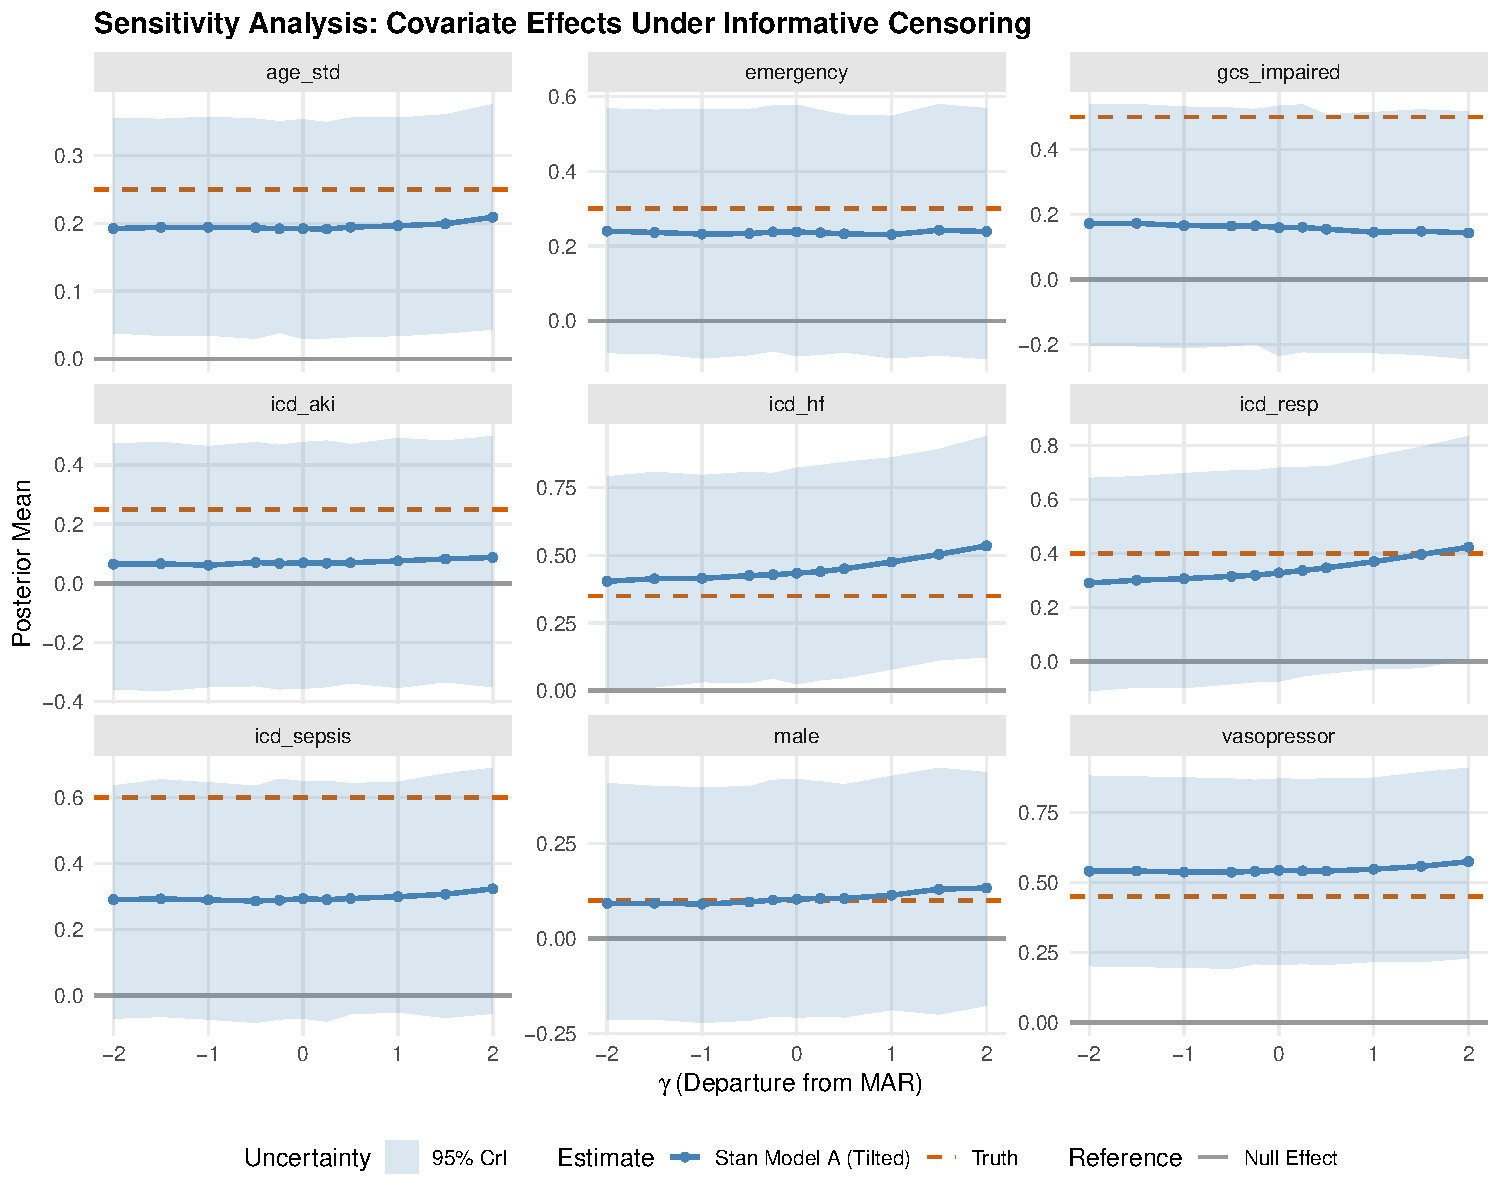
\includegraphics[width=0.8\textwidth]{plots/demo/stan_demo_sensitivity_all.pdf}
    \caption{Sensitivity analysis results showing posterior means and 95\% credible intervals for key covariate effects across a grid of \(\gamma\) values. Effects driven by observed covariates (e.g., age) remain stable, while those influenced by unobserved heterogeneity (e.g., sepsis) show sensitivity to informative censoring.}
\end{figure}


\paragraph{Discretization sensitivity.}
Covariate effects from Model~A are stable across \(\Delta \in \{1, 3, 7, 14\}\), while \(\hat{\sigma}_b\) from Model~B varies erratically (0.4 to 2.0), confirming that the frailty variance is not a stable estimand under different partitions of the same continuous-time process.


\paragraph{Calibration under informative censoring.} \label{fig:calibration}
The risk-decile calibration plot for Model~A shows systematic over-prediction of observed mortality, consistent with the bias formula \eqref{eq:bias-approx}. This confirms that the independent censoring assumption is violated in the simulation and that the bias manifests as miscalibration in the predicted risk quantiles.

\begin{figure}
    \centering
    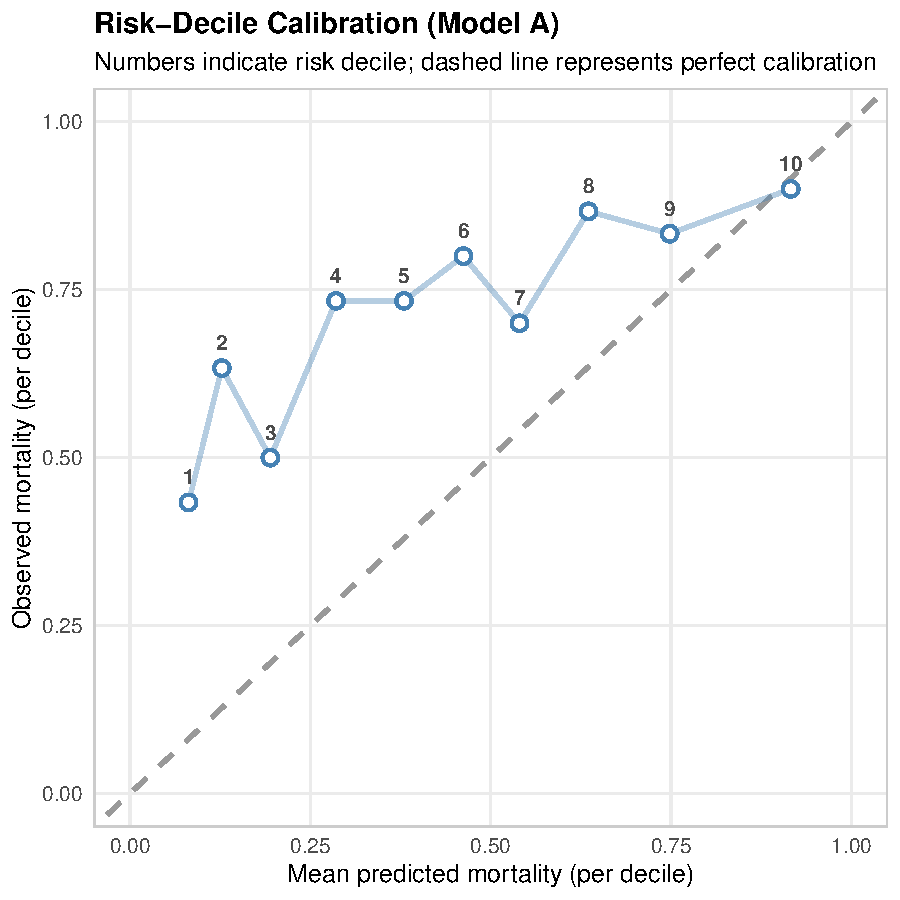
\includegraphics[width=0.7\textwidth]{plots/demo/stan_demo_calibration.pdf}
    \caption{Calibration plot for Model~A showing observed vs. predicted mortality across risk deciles. The systematic over-prediction in higher risk deciles confirms the presence of informative censoring bias, consistent with the theoretical bias formula.}
\end{figure}


\newpage 
\bibliography{references}

\end{document}
